\documentclass[11pt,a4paper]{article}
\usepackage[T1]{fontenc}
\usepackage[margin=2.3cm]{geometry}
\usepackage{amsmath,amssymb}
\usepackage{graphicx}
\usepackage[dvipsnames]{xcolor}
\usepackage{enumitem}
\usepackage[colorlinks=true,linkcolor=blue,urlcolor=blue]{hyperref}
\setlength{\parskip}{0.6em}
\setlength{\parindent}{0pt}
\begin{document}

\begin{center}{\LARGE\bfseries openorbit}\\[0.4em]{\large Plan a satellite transfer orbit with Kepler's laws, in three sessions.}\\[0.2em]\small PAN IIT OSS explainer \textbullet{} secondary school to diploma / undergraduate (levels 3-5)\end{center}

\section*{Why this exists}
Every satellite is a stone falling around the Earth. This explainer shows how Kepler's three laws, a single equation for speed, and a numerical check let you plan the cheapest simple way to move a satellite to a higher orbit.

\section*{The end goal}
Plan satellite transfer orbits with Kepler's laws. The end goal is planning satellite transfer orbits with Kepler's laws, as mission designers do for communication satellites, navigation constellations and space probes. The same mathematics drives space-station reboosts and the path of a probe to Mars.

\section*{How the three sessions build up}
\begin{enumerate}[nosep]
\item \textbf{Session 1: A satellite is falling around the Earth} (Level 1, conceptual interactive model, 60 min).
\item \textbf{Session 2: The mathematics of an orbit} (Level 2, mathematical engineering model, 75 min).
\item \textbf{Session 3: Plan a transfer orbit and check it} (Level 3, simulation and validation, 90 min).
\end{enumerate}

\section{Session 1: A satellite is falling around the Earth}

\subsection*{A. Real-world problem}
A satellite has no engine pushing it along, yet it stays up for years. Why does it not drop out of the sky? The answer is that it does fall, all the time, but it moves sideways so fast that the Earth curves away beneath it as quickly as it falls. How fast is that, and how long does one lap take? Why do the International Space Station and a weather satellite take such different times to go round? Educational model: a point satellite and a perfectly round Earth.

\subsection*{B. Concept and theory}
Gravity at distance r from the centre of the Earth gives every object the acceleration g = mu / r\textasciicircum{}2, where mu = 3.986004418e14 m\textasciicircum{}3/s\textasciicircum{}2 is the Earth's gravitational parameter. Fire a cannonball sideways at speed v: in time t it would travel a straight line d = v t while gravity pulls it down by about 0.5 g t\textasciicircum{}2, and the round ground curves away from the straight line by r - sqrt(r\textasciicircum{}2 - d\textasciicircum{}2). When these two are equal the cannonball keeps missing the ground: that speed is v = sqrt(mu / r), and one lap takes T = 2 pi r / v. Because gravity weakens with distance, v falls as r grows, and T grows even faster. Kepler found three laws that describe every orbit: (1) orbits are ellipses with the Earth at one focus; (2) the line from the Earth to the satellite sweeps equal areas in equal times, so the satellite is fast when close and slow when far; (3) T\textasciicircum{}2 divided by a\textasciicircum{}3 is the same for all orbits around the Earth, where a is the semi-major axis (the radius for a circle).

\begin{itemize}[nosep]
\item mu: Earth's gravitational parameter G times mass (m\textasciicircum{}3/s\textasciicircum{}2)
\item r: distance from the centre of the Earth (altitude plus 6371 km) (m)
\item g: gravity acceleration at distance r (m/s\textasciicircum{}2)
\item v: speed of the satellite (m/s)
\item T: time for one lap (period) (s)
\item a: semi-major axis: half the long side of the ellipse (m)
\end{itemize}

\begin{equation*}
g(r)=\frac{\mu}{r^{2}}
\end{equation*}

\begin{equation*}
v=\sqrt{\frac{\mu}{r}}
\end{equation*}

\begin{equation*}
T=\frac{2\pi r}{v}=2\pi\sqrt{\frac{r^{3}}{\mu}}
\end{equation*}

\begin{equation*}
\frac{T^{2}}{a^{3}}=\frac{4\pi^{2}}{\mu}\quad\text{(the same for every orbit)}
\end{equation*}

\begin{center}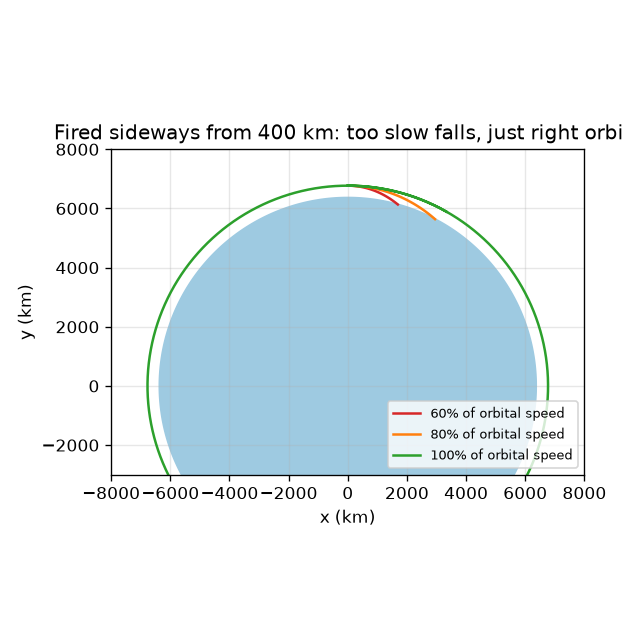
\includegraphics[width=0.85\linewidth]{figures/s01_falling_around.png}\\\small Fired sideways from 400 km: too slow and it falls to the ground, just right and it goes round.\end{center}

\subsection*{E. Worked example}
Find the speed, period and gravity for a satellite 400 km above the ground, and check that the Earth curves away as fast as the satellite falls in one second.
\begin{enumerate}[nosep]
\item Radius r = 6371 + 400 = 6771 km = 6.771e6 m.
\item Gravity g = mu / r\textasciicircum{}2 = 3.986e14 / (6.771e6)\textasciicircum{}2 = 8.69 m/s\textasciicircum{}2 (compare 9.82 m/s\textasciicircum{}2 at the surface).
\item Speed v = sqrt(mu / r) = 7.67 km/s.
\item Period T = 2 pi r / v = 2 pi * 6771 / 7.673 = 5545 s = 92.4 min.
\item In 1 s the satellite falls 0.5 * 8.69 * 1\textasciicircum{}2 = 4.35 m. In 1 s it moves 7.67 km sideways, and the circle of radius 6771 km drops away from a straight line by 6771 - sqrt(6771\textasciicircum{}2 - 7.67\textasciicircum{}2) km = 4.35 m. The two agree.
\end{enumerate}
\textbf{Answer.} v = 7.67 km/s, T = 92.4 min, g = 8.69 m/s\textasciicircum{}2, and fall and curve-away are both 4.35 m in one second.

\subsection*{F. Questions}
\begin{enumerate}[nosep]
\item \textbf{Conceptual.} Astronauts on the station float. Is gravity switched off up there? Explain what 'weightless' means.
\item \textbf{Numerical.} Find the speed and period of a circular orbit 1000 km above the ground. Check the sanity of your answer against the 400 km orbit.
\item \textbf{Graph and simulation interpretation.} In the speed and period graphs, what is the speed near 200 km and at the geostationary height, and what happens to the period? Why is the period curve steeper than the speed curve?
\item \textbf{Design and optimisation challenge.} Design: an Earth-observation satellite should go round once every 100 minutes in a circular orbit. At what altitude should it fly and how fast does it move? Is the answer reasonable for a real satellite?
\end{enumerate}

\section{Session 2: The mathematics of an orbit}

\subsection*{A. Real-world problem}
An operator needs an orbit that dips to 500 km above the ground and climbs to 35786 km. How long is one lap? How fast is the satellite at the lowest and highest point? And where is it one hour after passing the lowest point? A circular orbit cannot answer these questions: we need ellipses. Educational model: two bodies, no drag, no Earth bulge.

\subsection*{B. Concept and theory}
The closest point is the perigee (radius rp) and the farthest the apogee (radius ra), both measured from the Earth's centre. The semi-major axis is a = (rp + ra) / 2 and the eccentricity is e = (ra - rp) / (ra + rp); e = 0 is a circle. Kepler 3 gives the period T = 2 pi sqrt(a\textasciicircum{}3 / mu). The speed at distance r follows from the vis-viva equation v\textasciicircum{}2 = mu (2 / r - 1 / a). Along the orbit the energy per kilogram, v\textasciicircum{}2 / 2 - mu / r = -mu / (2 a), and the angular momentum r v (sideways part) are constant, which is Kepler 2: speed is inversely proportional to distance at perigee and apogee. To locate the satellite at time t, take the mean anomaly M = 2 pi t / T. It is connected to the eccentric anomaly E by Kepler's equation M = E - e sin E, which has no closed-form solution; Newton's method E \textless{}- E - (E - e sin E - M) / (1 - e cos E) solves it in a few steps, then r = a (1 - e cos E). To check the physics we also integrate the two-body equation, acceleration = -mu r / \textbar{}r\textbar{}\textasciicircum{}3, with RK4 (accurate steps, but energy error that drifts) and leapfrog (a symplectic method: energy error wobbles but does not grow).

\begin{itemize}[nosep]
\item rp, ra: perigee and apogee radius (m)
\item a: semi-major axis (m)
\item e: eccentricity (no unit)
\item T: period (s)
\item M: mean anomaly (steady clock angle) (rad)
\item E: eccentric anomaly (geometric angle) (rad)
\item h: specific angular momentum r v (m\textasciicircum{}2/s)
\item dt: integration time step (s)
\end{itemize}

\begin{equation*}
a=\frac{r_p+r_a}{2},\qquad e=\frac{r_a-r_p}{r_a+r_p},\qquad T=2\pi\sqrt{\frac{a^{3}}{\mu}}
\end{equation*}

\begin{equation*}
v^{2}=\mu\left(\frac{2}{r}-\frac{1}{a}\right)
\end{equation*}

\begin{equation*}
\varepsilon=\frac{v^{2}}{2}-\frac{\mu}{r}=-\frac{\mu}{2a},\qquad h=r_p v_p=r_a v_a
\end{equation*}

\begin{equation*}
M=\frac{2\pi t}{T}=E-e\sin E,\qquad E_{k+1}=E_k-\frac{E_k-e\sin E_k-M}{1-e\cos E_k},\qquad r=a(1-e\cos E)
\end{equation*}

\begin{center}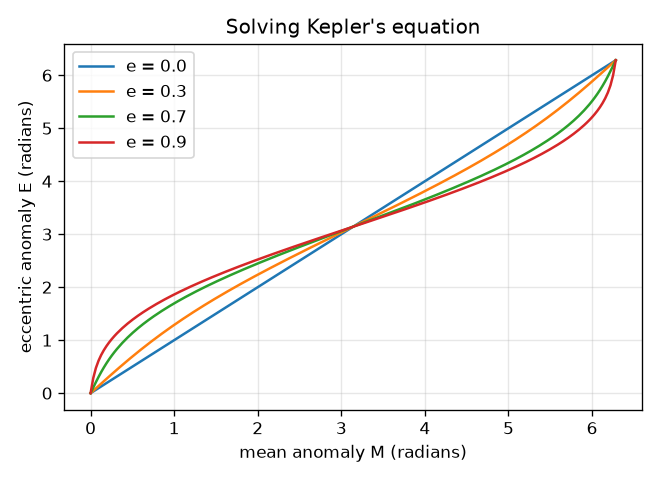
\includegraphics[width=0.85\linewidth]{figures/s02_kepler_equation.png}\\\small Eccentric anomaly E against mean anomaly M for several eccentricities.\end{center}

\subsection*{E. Worked example}
Design the orbit with perigee altitude 500 km and apogee altitude 35786 km. Find a, e, T, the speeds at perigee and apogee, and the satellite's distance one hour after perigee.
\begin{enumerate}[nosep]
\item rp = 6371 + 500 = 6871 km and ra = 6371 + 35786 = 42157 km.
\item a = (6871 + 42157) / 2 = 24514 km and e = (42157 - 6871) / (42157 + 6871) = 0.7197.
\item T = 2 pi sqrt(a\textasciicircum{}3 / mu) = 10.610 hours.
\item Vis-viva: perigee speed 9.988 km/s and apogee speed 1.628 km/s. Check with angular momentum: the ratio of the speeds is 6.135 and the ratio of the radii is 42157 / 6871 = 6.135.
\item Energy per kilogram = -mu / (2 a) = -8.13 MJ/kg at both ends.
\item One hour after perigee: M = 2 pi * 3600 / (10.610 * 3600) = 0.5922 rad. Newton's method gives E = 1.2821 rad in 5 iterations, so r = a (1 - e cos E) = 19491 km.
\end{enumerate}
\textbf{Answer.} a = 24514 km, e = 0.7197, T = 10.610 h, perigee speed 9.988 km/s, apogee speed 1.628 km/s, and r = 19491 km one hour after perigee (E = 1.2821 rad).

\subsection*{F. Questions}
\begin{enumerate}[nosep]
\item \textbf{Conceptual.} Why must a satellite move faster at perigee than at apogee? Answer using both energy and angular momentum.
\item \textbf{Numerical.} Use Kepler's third law to find the period of an orbit with semi-major axis 24514 km. Check units and compare with the geostationary period.
\item \textbf{Graph and simulation interpretation.} From the energy figure, which integrator would you trust for a simulation of 1000 laps, and why? Which is more accurate for 10 laps?
\item \textbf{Design and optimisation challenge.} Design: you need a 12 hour orbit that passes 500 km above the ground at perigee. What apogee altitude do you need, and what is the semi-major axis? How would you choose between this orbit and a circular one with the same period?
\end{enumerate}

\section{Session 3: Plan a transfer orbit and check it}

\subsection*{A. Real-world problem}
A satellite is released into a low circular orbit and must reach the geostationary orbit. Fuel is the scarcest thing on board, so every metre per second of speed change (delta-v) costs mass. What is the cheapest simple way, how long does it take, and how do we know the plan really works? Educational model: instant burns, two bodies, circular coplanar orbits. This is not a mission design tool.

\subsection*{B. Concept and theory}
A Hohmann transfer uses an ellipse that touches the inner circle (radius r1) at its perigee and the outer circle (radius r2) at its apogee: its semi-major axis is a\_t = (r1 + r2) / 2. Burn 1 at r1 raises the speed from the circular speed to the ellipse's perigee speed; burn 2 at r2 raises it from the ellipse's apogee speed to the circular speed; both come from vis-viva. The flight takes half the period of the ellipse. A bi-elliptic transfer goes out to a far radius rb, then in to r2: three burns. For a radius ratio r2 / r1 above about 11.94 it can cost less delta-v than Hohmann, but takes much longer. Turning the velocity by an angle di without changing speed costs 2 v sin(di / 2), cheapest where v is smallest, so a plane change belongs at the apogee of the transfer, combined with the second burn at the cost sqrt(v1\textasciicircum{}2 + v2\textasciicircum{}2 - 2 v1 v2 cos di). The Oberth effect: adding delta-v to speed v adds energy v dv + dv\textasciicircum{}2 / 2 per kilogram, so the same dv gives more energy when v is high. Phasing: a chaser in a lower orbit has the higher angular rate n = sqrt(mu / r\textasciicircum{}3) and catches a target lead\_deg ahead after lead / (n1 - n2). Finally, real burns take time: a weak engine burning for many minutes wastes some push as the satellite climbs (gravity loss).

\begin{itemize}[nosep]
\item r1, r2: radii of the inner and outer circular orbits (m)
\item a\_t: semi-major axis of the transfer ellipse (m)
\item dv1, dv2: the two burns (m/s)
\item rb: apogee radius of the bi-elliptic transfer (m)
\item di: plane change angle (degrees)
\item n: angular rate sqrt(mu / r\textasciicircum{}3) (rad/s)
\item dt: integration step (s)
\end{itemize}

\begin{equation*}
a_t=\frac{r_1+r_2}{2},\qquad \Delta v_1=\sqrt{\mu\left(\frac{2}{r_1}-\frac{1}{a_t}\right)}-\sqrt{\frac{\mu}{r_1}},\qquad \Delta v_2=\sqrt{\frac{\mu}{r_2}}-\sqrt{\mu\left(\frac{2}{r_2}-\frac{1}{a_t}\right)}
\end{equation*}

\begin{equation*}
t_{\text{transfer}}=\pi\sqrt{\frac{a_t^{3}}{\mu}}
\end{equation*}

\begin{equation*}
\Delta v_{\text{plane}}=2v\sin\frac{\Delta i}{2},\qquad \Delta v_{\text{combined}}=\sqrt{v_1^{2}+v_2^{2}-2v_1v_2\cos\Delta i}
\end{equation*}

\begin{equation*}
\Delta\varepsilon=v\,\Delta v+\frac{\Delta v^{2}}{2},\qquad t_{\text{phase}}=\frac{\varphi}{n_1-n_2}
\end{equation*}

\begin{center}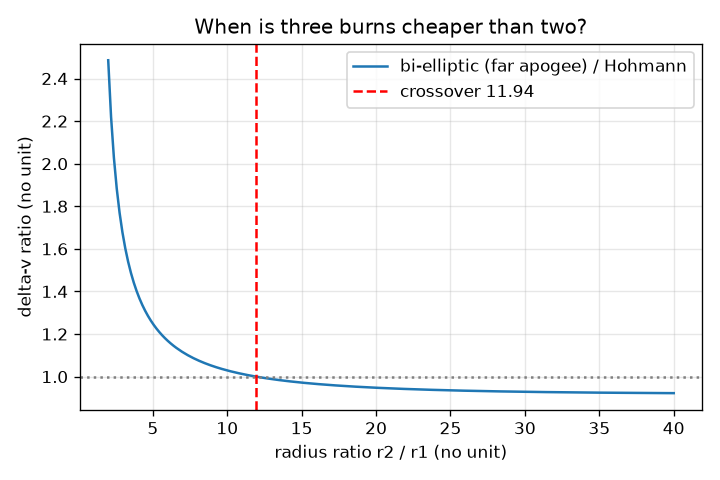
\includegraphics[width=0.85\linewidth]{figures/s03_bielliptic_vs_hohmann.png}\\\small Bi-elliptic delta-v divided by Hohmann delta-v: crossover at a radius ratio of about 11.94.\end{center}

\subsection*{E. Worked example}
Plan the Hohmann transfer from a circular orbit of radius 6778 km (a low orbit) to the geostationary radius 42164 km. Find both burns, the total, and the flight time, and verify them by integration.
\begin{enumerate}[nosep]
\item a\_t = (6778 + 42164) / 2 = 24471 km.
\item Speeds: circular at 6778 km is 7.669 km/s, the transfer's perigee speed is 10.066 km/s, the transfer's apogee speed is 1.618 km/s, and the circular speed at 42164 km is 3.075 km/s.
\item dv1 = 10.066 - 7.669 = 2.398 km/s. dv2 = 3.075 - 1.618 = 1.457 km/s. Total = 3.854 km/s.
\item Transfer time = half the period of the ellipse = 5.291 hours.
\item Numerical check: start at 6778 km, speed 10.066 km/s, integrate for 5.291 hours with RK4. The satellite arrives at radius 42164 km (within 1 km), on the opposite side of the Earth (180 degrees), moving at 1618 m/s. After adding dv2 the orbit stays circular to within 1 m for a whole lap.
\end{enumerate}
\textbf{Answer.} dv1 = 2.398 km/s, dv2 = 1.457 km/s, total 3.854 km/s (about 3.9), flight time 5.291 h (about 5.3 h), confirmed by integration to within 1 km.

\subsection*{F. Questions}
\begin{enumerate}[nosep]
\item \textbf{Conceptual.} Why are both Hohmann burns along the velocity (tangential), and why is the flight time half an ellipse period?
\item \textbf{Numerical.} Find the Hohmann burns and the transfer time between the circular orbits of radius 6778 km and 7178 km (a small step, for example before docking).
\item \textbf{Graph and simulation interpretation.} In the bi-elliptic graph, for which radius ratios is Hohmann cheaper, and what does the 11.94 crossing mean for LEO to GEO?
\item \textbf{Design and optimisation challenge.} Design: a satellite is launched into a low orbit inclined 28.5 degrees and must be put into the equatorial geostationary orbit. Compare three plans for the plane change: in the low orbit, at the geostationary orbit, and combined with the second burn at the transfer apogee. Which would you choose and what is the trade-off?
\end{enumerate}

\section{Real-world mini-project}
\textbf{Plan a transfer from a 500 km orbit to a 20200 km orbit.} A navigation satellite is released into a circular orbit 500 km above the ground and must reach a circular orbit 20200 km above the ground. Use \texttt{hohmann} and \texttt{check\_hohmann} from Session 3 (altitudes are measured from the ground, so add the Earth radius 6371 km to get orbit radii). Report both burns, the transfer time, and the result of the numerical check. Also show that a bi-elliptic route with an apogee of three times the final radius is more expensive here.

\section{The path ahead}
\begin{enumerate}[nosep]
\item \textbf{Session 4: Split the plane change between burns.} A planner that divides the 28.5 degree turn between the two burns of the GEO transfer and finds the best split.
\item \textbf{Session 5: Full rendezvous.} A planner that takes a chaser and a target in circular orbits with a starting angle and returns the burns and the time to meet.
\item \textbf{Session 6: Orbit plane drift (J2).} An integrator in 3D with the J2 term added to the acceleration.
\item \textbf{Session 7: Low-thrust spiral.} A guidance law that steers continuous thrust along the velocity and stops at the target radius.
\item \textbf{Session 8: Earth to Mars.} A heliocentric planner with the Sun's gravitational parameter and circular planet orbits.
\end{enumerate}

\section{Answers and hints}

\subsection*{Session 1}
\begin{enumerate}[nosep]
\item \textbf{Conceptual.} Hint: Compare gravity at 400 km with the surface value, and think about falling together. Solution: No. Gravity at 400 km is 8.69 m/s\textasciicircum{}2, compared with 9.82 m/s\textasciicircum{}2 at the surface, so it is still strong. The astronauts and the station fall together around the Earth with the same acceleration, so nothing pushes them against the floor. They feel weightless because they are in free fall, not because gravity is absent.
\item \textbf{Numerical.} Hint: r = 6371 + 1000 km. Use v = sqrt(mu / r) and T = 2 pi r / v. Solution: r = 7371 km. v = 7.35 km/s and T = 105.0 min. Sanity check: higher than the 400 km orbit, so slower (7.35 below 7.67 km/s) and a longer period (105.0 above 92.4 min). Units: km/s and minutes.
\item \textbf{Graph and simulation interpretation.} Hint: Read the left and right ends of both curves. Remember T = 2 pi r / v. Solution: At 200 km: 7.79 km/s and a period of 88.4 min. At 35786 km: 3.07 km/s and a period of 1435.7 min, about 23.93 hours. The period grows for two reasons at once: the path 2 pi r is longer, and the speed v is lower, so the period changes faster than either alone.
\item \textbf{Design and optimisation challenge.} Hint: Solve Kepler 3 for the radius: r = (mu (T / 2 pi)\textasciicircum{}2)\textasciicircum{}(1/3) with T = 6000 s. Solution: r gives an altitude of 765.6 km and a speed of 7.473 km/s. This is reasonable: it is in the range of real imaging satellites, above most of the thin air that slows lower orbits. Trade-off: higher means longer lap and a wider view but a smaller picture detail; lower means sharper pictures but more drag.
\end{enumerate}

\subsection*{Session 2}
\begin{enumerate}[nosep]
\item \textbf{Conceptual.} Hint: Compare v\textasciicircum{}2 / 2 - mu / r at two radii, and r v at two radii. Solution: Angular momentum h = r v is constant, so the product of radius and speed is the same at both ends: the smaller radius needs the bigger speed (the ratio of speeds equals the inverse ratio of radii, 6.135 in the worked example). In terms of energy, the satellite gains kinetic energy as it falls toward the Earth, trading it for potential energy, while the total -mu / (2 a) stays constant.
\item \textbf{Numerical.} Hint: T = 2 pi sqrt(a\textasciicircum{}3 / mu), with a in metres. Solution: T = 10.610 hours. Units: metres cubed over metres cubed per second squared gives seconds squared; its root is seconds. Sanity check: smaller than the 23.93 hours at 42164 km because the semi-major axis is smaller; Kepler 3 says period grows as a\textasciicircum{}1.5.
\item \textbf{Graph and simulation interpretation.} Hint: Look at whether each curve keeps growing or stays in a band. Solution: For very long runs, leapfrog: its energy error stays inside a band below 2e-3 and does not grow, and it conserves angular momentum to 1e-12. RK4's error is smaller at first (1.9e-6 after 10 laps) but grows steadily with the number of laps (7.8e-6 after 40), so over enough laps it eventually exceeds the band. The best choice depends on the number of laps and on whether a bounded error matters more than a small one.
\item \textbf{Design and optimisation challenge.} Hint: Solve Kepler 3 for a, then ra = 2a - rp. Solution: A period of 43200 s gives a = 26610 km, so the apogee altitude is 39978 km (apogee radius 2a - rp). A circular orbit with the same period would sit at one altitude all the time. The ellipse lingers for hours near its high point and covers the high latitudes, but flies through more radiation and needs more fuel to reach. Trade-off: coverage and dwell time versus launch cost and radiation.
\end{enumerate}

\subsection*{Session 3}
\begin{enumerate}[nosep]
\item \textbf{Conceptual.} Hint: The transfer ellipse touches both circles at its two ends; think about the directions of the velocities there. Solution: The ellipse is tangent to both circles at perigee and apogee, where the velocity is perpendicular to the radius for both curves. So the speed must change in size, not direction, which is a tangential burn. The satellite goes from perigee to apogee, which is half the ellipse and so half its period.
\item \textbf{Numerical.} Hint: a\_t = (r1 + r2) / 2, then use vis-viva as in the worked example. Solution: dv1 = 109.1 m/s, dv2 = 107.6 m/s, total 216.7 m/s, transfer time 2900.5 s. Sanity check: a 400 km step costs little, and the two burns are nearly equal. Units: metres per second and seconds.
\item \textbf{Graph and simulation interpretation.} Hint: Read where the curve is above and below 1 and compute the LEO to GEO ratio. Solution: Hohmann is cheaper to the left of 11.94 (the ratio 5 costs 1.249 times more with a bi-elliptic transfer, and 10 costs 1.029 times more); bi-elliptic is cheaper to the right (0.972 at 15). LEO to GEO has a ratio of 42164 / 6778 = 6.22, which is to the left, so Hohmann wins: a bi-elliptic with an apogee of 20 r2 costs 4.427 km/s and takes 32.9 days, against 3.854 km/s and 5.291 hours.
\item \textbf{Design and optimisation challenge.} Hint: Use 2 v sin(di / 2) with v = 7.669, 3.075 km/s, and the combined formula with 1.618 and 3.075 km/s. Solution: Turn in the low orbit: 3.775 km/s + 3.854 km/s = 7.629 km/s. Turn at the geostationary orbit: 3.854 + 1.514 = 5.368 km/s. Combined at apogee: 2.398 + 1.824 = 4.222 km/s. Combine with the second burn: the turn is done where the speed is lowest (1.618 km/s) and the burn serves two purposes at once. Trade-off: the one-burn plan needs the engine to point away from the velocity, and any error in direction misses the target plane, so a real plan often splits the turn between burns.
\end{enumerate}

\section{How to join}
Read \texttt{CONTRIBUTING.md} in the repository, then pick an issue labelled \texttt{good first issue}. Repository: \url{https://github.com/KrunalPanchal1995/openorbit}

\end{document}
